\documentclass[11pt,a4paper]{article}

\usepackage[margin=1in]{geometry}
\usepackage{graphicx}
\usepackage{booktabs}
\usepackage{array}
\usepackage{caption}
\usepackage{subcaption}
\usepackage{xcolor}
\usepackage{listings}
\usepackage{amsmath}
\usepackage{enumitem}
\usepackage{fancyhdr}
\usepackage{titlesec}
\usepackage[hidelinks]{hyperref}

\definecolor{codebg}{RGB}{245,245,245}
\definecolor{codekw}{RGB}{0,80,150}
\definecolor{codecomment}{RGB}{110,110,110}
\definecolor{codestring}{RGB}{140,20,20}

\lstset{
  backgroundcolor=\color{codebg},
  basicstyle=\ttfamily\small,
  keywordstyle=\color{codekw}\bfseries,
  commentstyle=\color{codecomment}\itshape,
  stringstyle=\color{codestring},
  showstringspaces=false,
  breaklines=true,
  frame=single,
  rulecolor=\color{gray!40},
  numbers=left,
  numberstyle=\tiny\color{gray},
  xleftmargin=1.8em,
  language=Python
}

\titleformat{\section}{\normalfont\Large\bfseries}{\thesection}{1em}{}
\titleformat{\subsection}{\normalfont\large\bfseries}{\thesubsection}{1em}{}

\pagestyle{fancy}
\fancyhf{}
\fancyhead[L]{ICS1512 -- Machine Learning Algorithms Laboratory}
\fancyhead[R]{Experiment 9}
\fancyfoot[C]{\thepage}
\renewcommand{\headrulewidth}{0.4pt}

\title{}
\date{}

\begin{document}

% ---------------- Title Page ----------------
\begin{titlepage}
\centering
\vspace*{1cm}
{\Large\bfseries Sri Sivasubramaniya Nadar College of Engineering, Chennai\par}
\vspace{0.2cm}
{\normalsize (An Autonomous Institution Affiliated to Anna University)\par}
\vspace{1.2cm}

{\Large\bfseries Machine Learning Algorithms Laboratory\par}
\vspace{0.3cm}
{\large ICS1512\par}
\vspace{1.5cm}

\begin{tabular}{|p{5.5cm}|p{7cm}|}
\hline
Degree \& Branch & M.Tech (Integrated) Computer Science \& Engineering \\
\hline
Semester & V \\
\hline
Academic Year & 2026--2027 (Odd) \\
\hline
Batch & 2024--2029 \\
\hline
\end{tabular}

\vspace{1.8cm}
{\Large\bfseries Experiment 9\par}
\vspace{0.3cm}
{\large Perceptron vs Multilayer Perceptron (A/B Experiment) with Hyperparameter Tuning\footnote{\textbf{GitHub Repository: }\url{https://github.com/VijayaraaghavanKS/ML}}\par}
\vspace{2.5cm}

\begin{tabular}{ll}
Submitted by: & \textbf{Vijayaraaghavan K S} \\[4pt]
Register Number: & \textbf{3122247001066} \\[4pt]
Year: & III Year \\[4pt]
Programme: & M.Tech Integrated, CSE \\[4pt]
Faculty: & Dr. Poreddy Ajay Kumar Reddy \\[4pt]
\end{tabular}

\vfill
\end{titlepage}

\tableofcontents
\newpage

% ==========================================================
\section{Aim and Objective}
To implement a single-layer Perceptron Learning Algorithm (PLA) from scratch and a tuned Multilayer Perceptron (MLP), compare their performance on the Kaggle English Handwritten Characters dataset (62 classes: 0--9, A--Z, a--z), and select and justify MLP hyperparameters (activation, optimizer, learning rate, hidden layers, batch size) through systematic tuning.

% ==========================================================
\section{Theory}
\textbf{PLA} uses a step activation and the update rule $w_{t+1} = w_t + \eta(y-\hat y)x$, adjusting weights only on misclassified samples; it converges only for linearly separable data and represents a linear decision boundary. Since PLA is inherently binary, this experiment extends it to 62 classes via a \textbf{one-vs-rest ensemble of 62 independent Perceptrons}, one per character, each trained with the same update rule; the class whose Perceptron gives the highest raw (pre-step) score is predicted. \textbf{MLP} stacks Input $\to$ Hidden Layer(s) $\to$ Output with nonlinear activations (ReLU, Sigmoid, Tanh), trained via backpropagation with a cross-entropy loss and a gradient-based optimizer (SGD, Adam); hidden layers let it learn non-linear decision boundaries a single-layer Perceptron cannot represent.

% ==========================================================
\section{Dataset and Preprocessing}
The dataset contains 3,410 images of handwritten characters across 62 classes (digits 0--9, uppercase A--Z, lowercase a--z), 55 images per class. Each image was converted to grayscale, resized to $32\times32$, flattened to a 1,024-dimensional vector, and normalized to $[0,1]$. An 80/20 stratified train/test split gave 2,728 training and 682 test images; a further 80/20 split of the training set was used to validate MLP hyperparameters.

\begin{figure}[h]
\centering
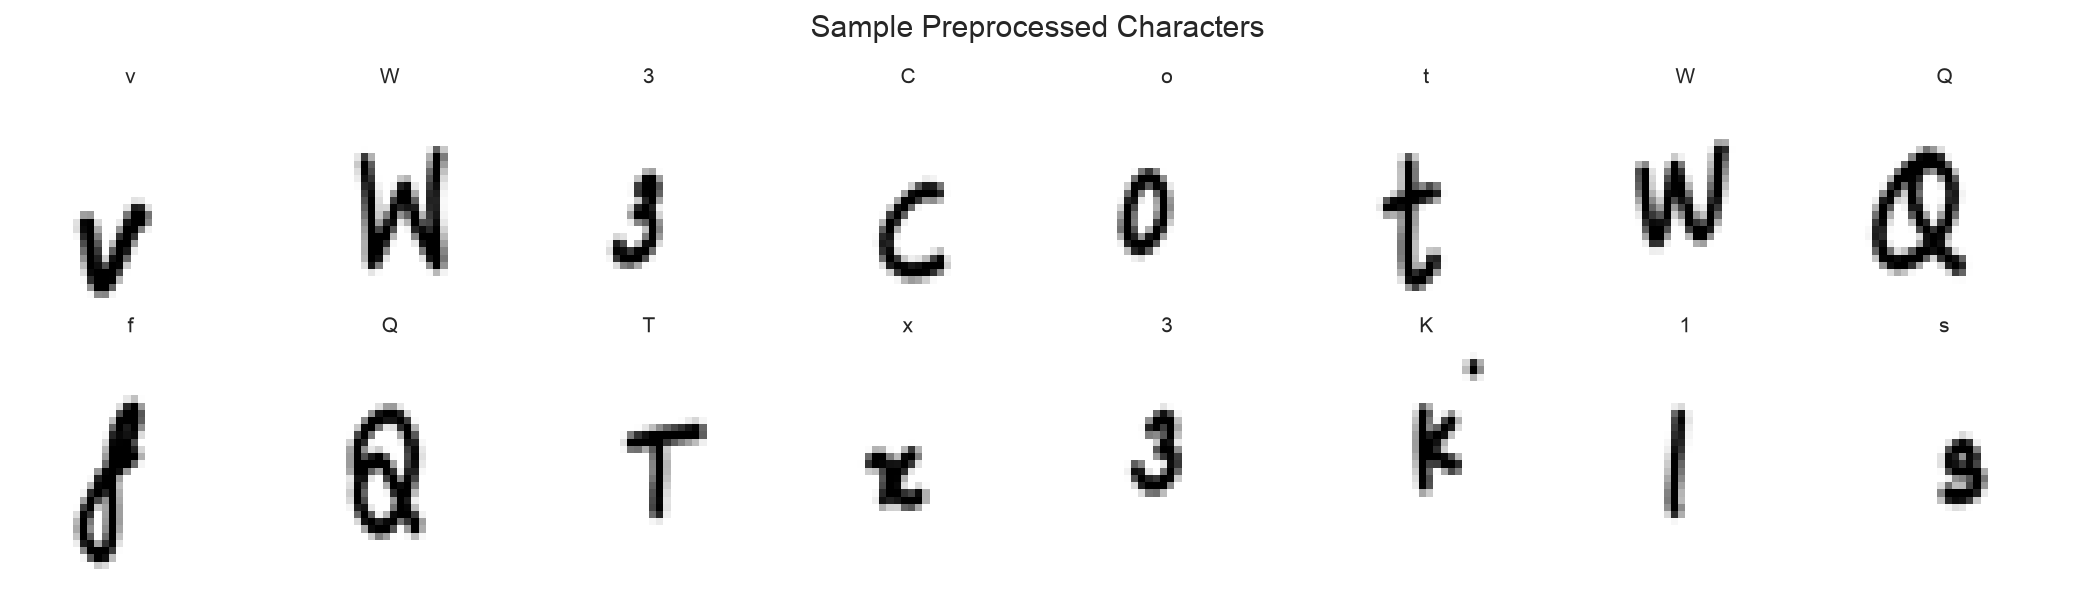
\includegraphics[width=0.85\linewidth]{experiment9_output/plots/sample_preprocessed_characters.png}
\caption{Sample preprocessed characters (32$\times$32 grayscale) with their class labels.}
\end{figure}

% ==========================================================
\section{Model A: PLA Implementation and Results}
PLA was implemented from scratch in NumPy as a one-vs-rest ensemble: 62 weight vectors, step activation, learning rate $\eta=0.01$, 50 epochs, with weights updated sample-by-sample using $w_{t+1}=w_t+\eta(y-\hat y)x$ against a $+1/-1$ target for each class.

\begin{figure}[h]
\centering
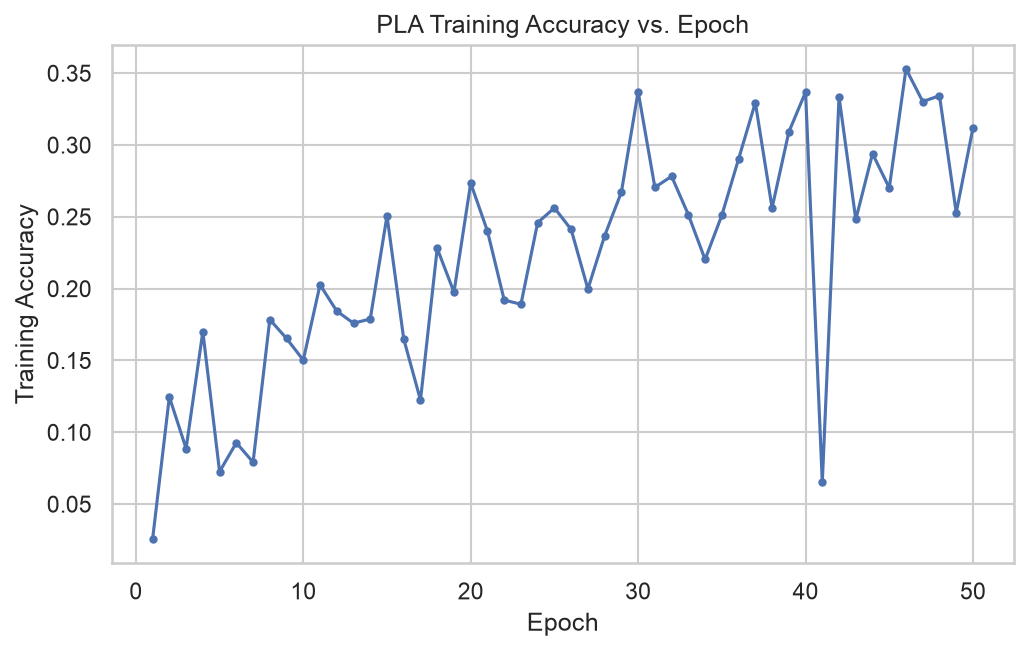
\includegraphics[width=0.6\linewidth]{experiment9_output/plots/pla_training_curve.png}
\caption{PLA training accuracy vs.\ epoch (one-vs-rest ensemble).}
\end{figure}
Training accuracy climbs steadily but plateaus well below 100\%, confirming the 62-class raw-pixel data is not linearly separable, so PLA cannot drive its training error to zero the way it could on a linearly separable two-class problem.

% ==========================================================
\section{Model B: MLP Implementation, Tuning, and Results}
\begin{table}[h]
\centering
\small
\begin{tabular}{@{}lllrrrrr@{}}
\toprule
Hidden Layers & Activation & Solver & LR & Batch & Val Acc & Time (s) & Iters \\
\midrule
\textbf{(256, 128)} & \textbf{relu} & \textbf{adam} & \textbf{0.001} & \textbf{64} & \textbf{0.4469} & 8.17 & 300 \\
(128,) & tanh & adam & 0.001 & 64 & 0.3059 & 4.03 & 300 \\
(128, 64) & relu & sgd & 0.01 & 64 & 0.3059 & 2.65 & 284 \\
(128, 64) & relu & adam & 0.001 & 64 & 0.2894 & 4.51 & 300 \\
(128, 64) & relu & adam & 0.001 & 128 & 0.1300 & 2.70 & 300 \\
(128, 64) & relu & adam & 0.01 & 64 & 0.0165 & 0.83 & 56 \\
(128,) & relu & adam & 0.001 & 64 & 0.0147 & 2.04 & 148 \\
(128, 64, 32) & relu & adam & 0.001 & 64 & 0.0147 & 2.86 & 181 \\
\bottomrule
\end{tabular}
\caption{MLP hyperparameter search over architecture, activation, optimizer, learning rate, and batch size.}
\end{table}
\textbf{Selected hyperparameters: hidden\_layer\_sizes=(256, 128), activation=ReLU, optimizer=Adam, learning\_rate=0.001, batch\_size=64} -- the only configuration that both trained for the full 300 iterations without stalling and reached a validation accuracy clearly above chance (1/62 $\approx$ 0.016). Half the grid collapsed to near-random accuracy, showing MLP training on this small, high-class-count dataset is unstable without a wide enough hidden layer and a moderate batch size.

\begin{figure}[h]
\centering
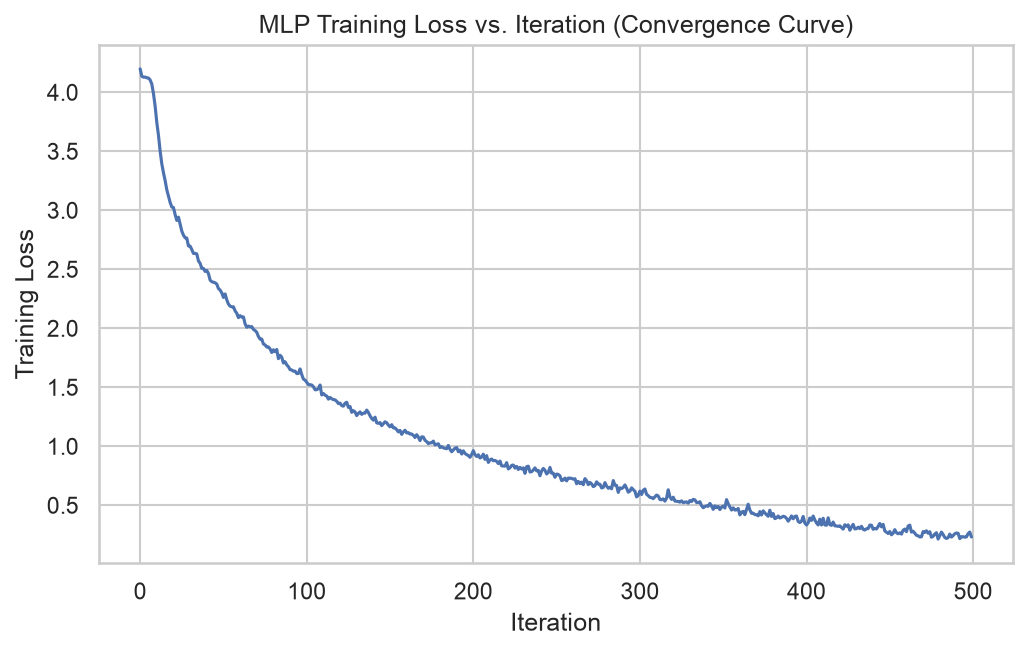
\includegraphics[width=0.6\linewidth]{experiment9_output/plots/mlp_training_curve.png}
\caption{Final MLP (256, 128) training loss vs.\ iteration.}
\end{figure}

% ==========================================================
\section{A/B Comparison: PLA vs.\ MLP}
\begin{table}[h]
\centering
\footnotesize
\begin{tabular}{@{}p{2.6cm}rrrrrrrr@{}}
\toprule
Model & Train Acc & Test Acc & Prec. & Recall & F1 & AUC-mi & AUC-ma & Time (s) \\
\midrule
PLA (1-vs-rest) & 0.3120 & 0.1804 & 0.3169 & 0.1804 & 0.1537 & 0.7947 & 0.8505 & 7.39 \\
MLP (256, 128) & 0.9652 & \textbf{0.4355} & \textbf{0.4598} & \textbf{0.4355} & \textbf{0.4355} & \textbf{0.9382} & \textbf{0.9385} & 16.74 \\
\bottomrule
\end{tabular}
\caption{PLA vs.\ tuned MLP, all metrics macro-averaged over 62 classes where applicable (AUC-mi/ma = micro/macro-averaged ROC-AUC).}
\end{table}

\begin{figure}[h]
\centering
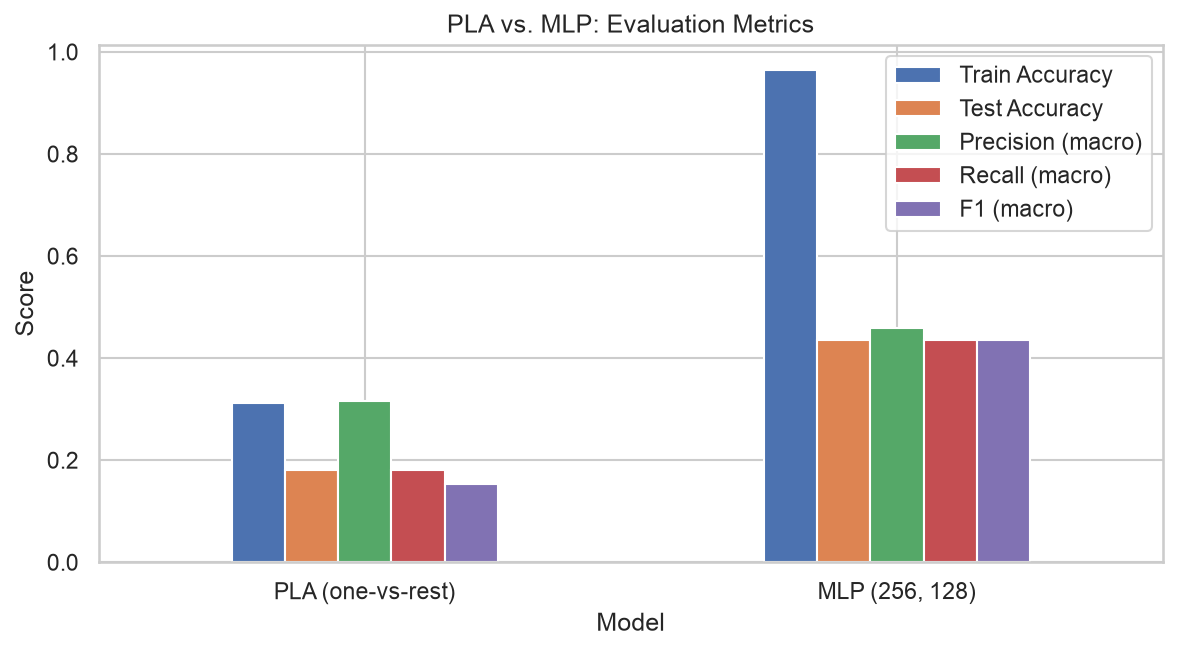
\includegraphics[width=0.85\linewidth]{experiment9_output/plots/ab_comparison_bar_plot.png}
\caption{PLA vs.\ MLP across accuracy, precision, recall, and F1.}
\end{figure}

\textbf{Strengths/weaknesses:} PLA is simple, fast (7.4s), and interpretable, but its purely linear decision boundary caps test accuracy at 0.1804 -- barely above 10$\times$ random guessing (1/62). MLP more than doubles PLA's test accuracy and macro-F1 by learning non-linear boundaries through its hidden layers, at the cost of a much larger train-test accuracy gap (Section 7) and roughly 2.3$\times$ the training time.

\begin{figure}[h]
\centering
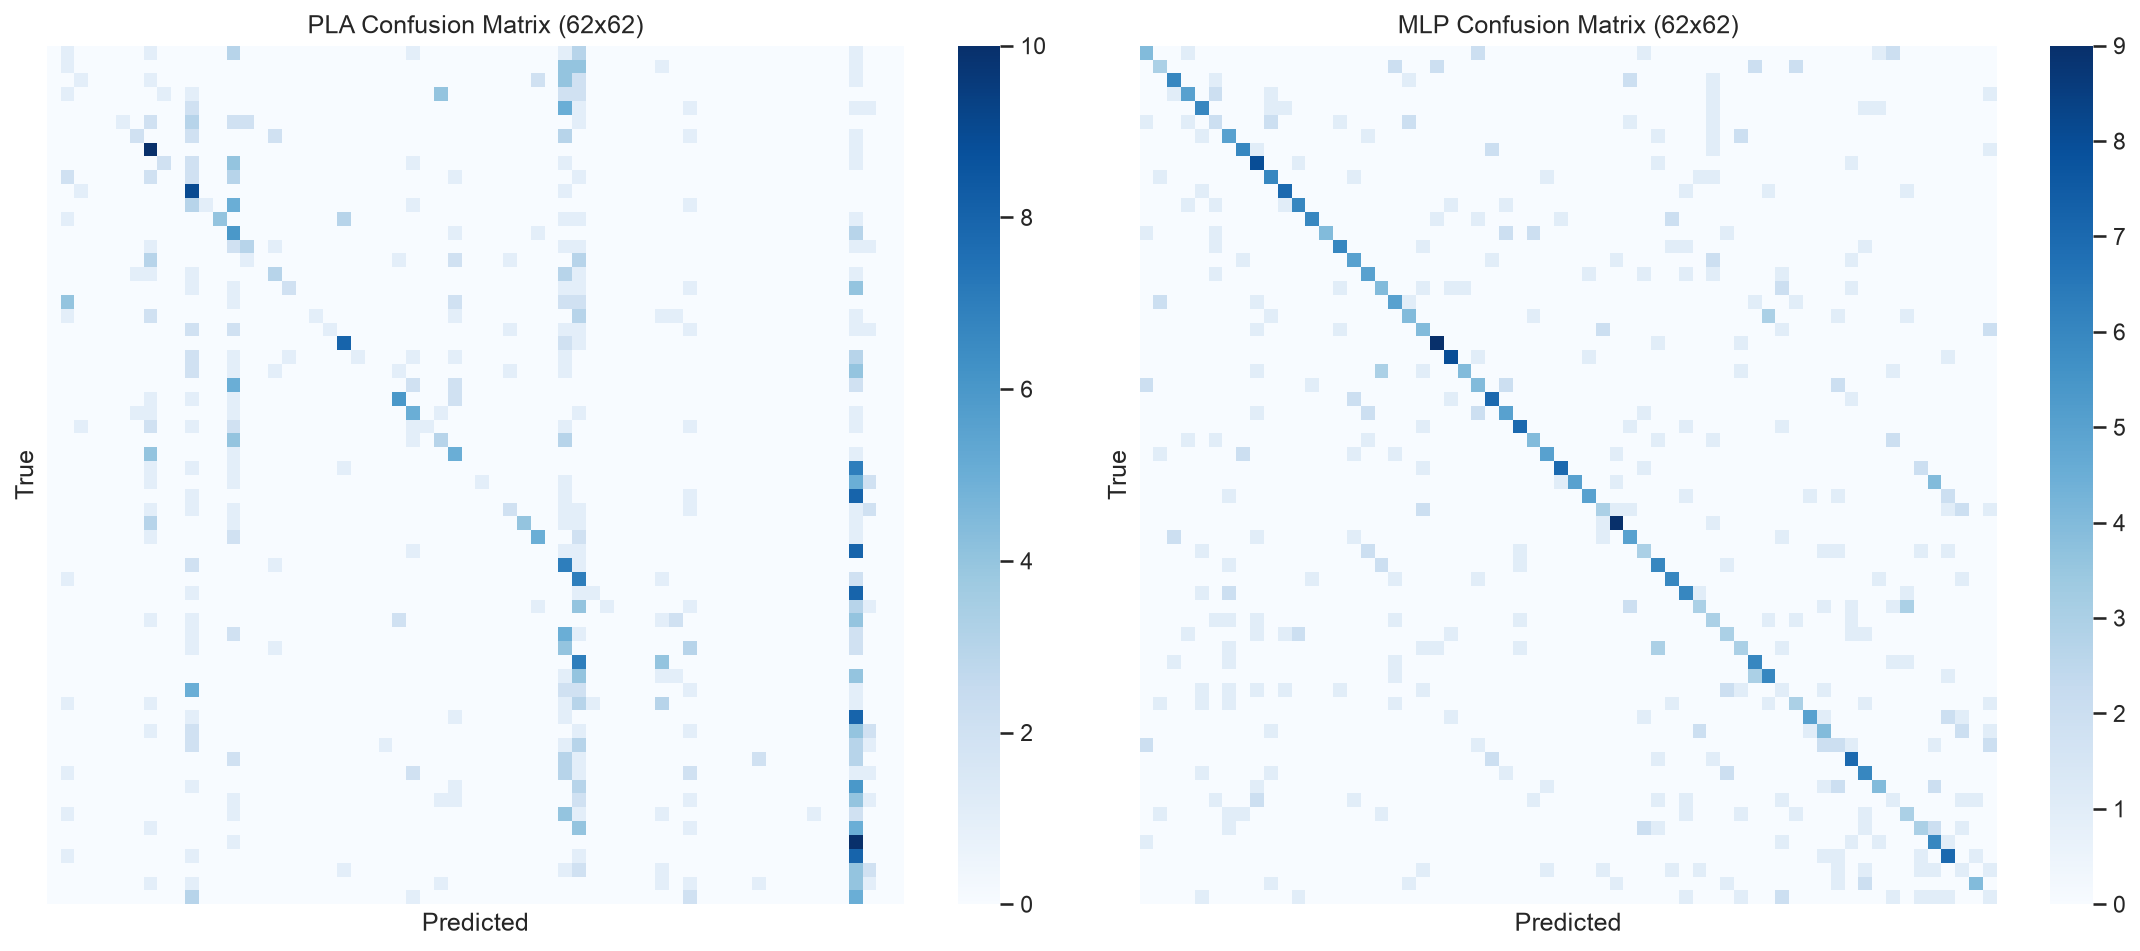
\includegraphics[width=0.85\linewidth]{experiment9_output/plots/confusion_matrices.png}
\caption{Confusion matrices (62$\times$62, unannotated heatmap): PLA (left) vs.\ MLP (right). MLP's diagonal is visibly denser.}
\end{figure}

\begin{figure}[h]
\centering
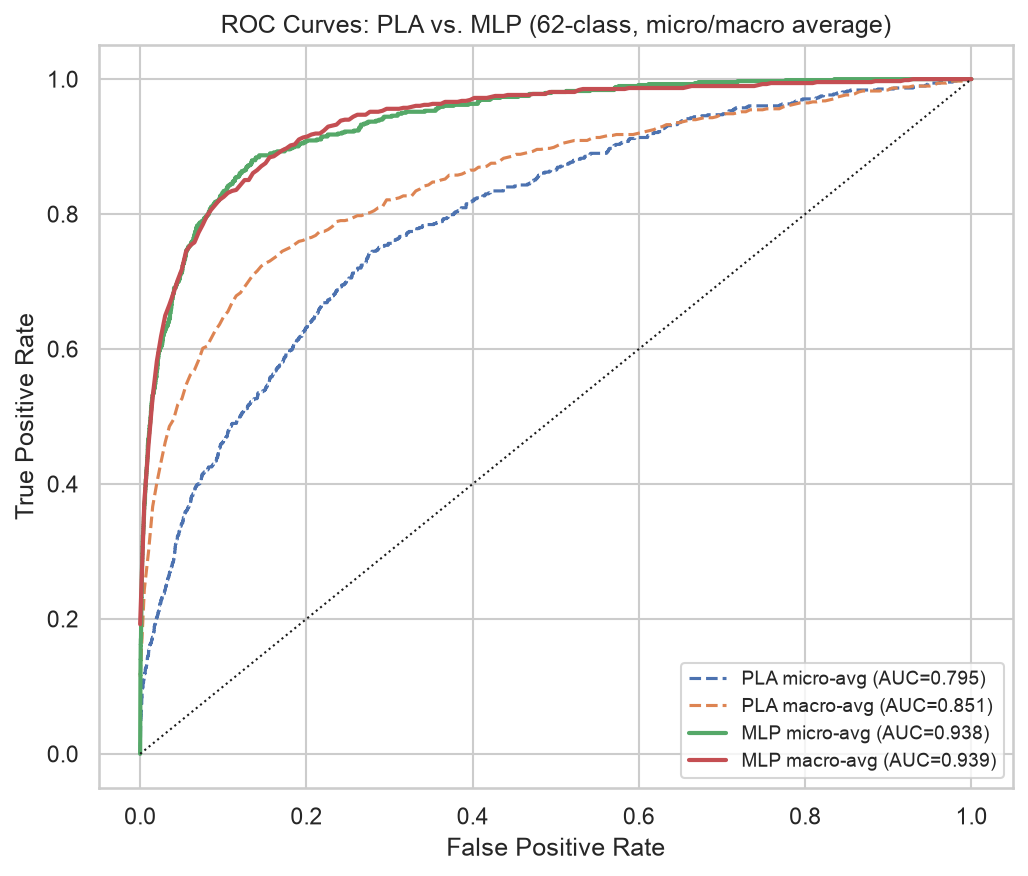
\includegraphics[width=0.75\linewidth]{experiment9_output/plots/roc_curves_pla_vs_mlp.png}
\caption{Micro/macro-averaged ROC curves, PLA vs.\ MLP.}
\end{figure}

% ==========================================================
\section{Overfitting Analysis}
MLP's train-test accuracy gap is $0.9652-0.4355=0.5297$, far larger than PLA's gap of $0.3120-0.1804=0.1316$. This is expected given only $2728/62 \approx 44$ training images per class for a 62-way classification problem -- the (256, 128) network has far more parameters than can be reliably fit from that little data per class. Mitigation options include stronger L2 regularization (\texttt{alpha}), early stopping on a validation set, or, most effectively, data augmentation (small rotations/shifts/noise) to increase the effective number of training examples per class.

% ==========================================================
\section{Observation Questions}

\textbf{Why does PLA underperform compared to MLP?}\\
PLA reaches 0.1804 test accuracy versus MLP's 0.4355 because PLA can only draw a linear decision boundary per class, while 62-way handwritten character recognition on raw pixels is not linearly separable -- many characters (e.g.\ visually similar digits, upper/lowercase pairs) need a non-linear boundary only MLP's hidden layers can represent.

\textbf{Which hyperparameters had the most impact on MLP performance?}\\
Hidden layer size/depth and optimizer choice mattered most: the best (256, 128)/Adam configuration reached 0.4469 validation accuracy versus SGD's 0.3059 at the same depth, a larger gap than switching activation alone (ReLU vs.\ Tanh differed by only 0.0165 at the smaller architecture).

\textbf{Did optimizer choice (SGD vs Adam) affect convergence?}\\
Yes: Adam configurations converged in 226 iterations on average vs.\ 284 for SGD, and the best Adam run's validation accuracy was notably higher, consistent with Adam's per-parameter adaptive learning rates converging faster and more reliably than plain SGD here.

\textbf{Did adding more hidden layers always improve results? Why or why not?}\\
No: the 3-hidden-layer (128, 64, 32) network reached only 0.0147 validation accuracy, far below the 2-hidden-layer (128, 64) network's 0.3059. With only $\approx$35 samples/class in the tuning split, a deeper network has more parameters than the data can reliably fit, so added depth made optimization harder instead of improving accuracy.

\textbf{Did MLP show overfitting? How could it be mitigated?}\\
Yes, clearly (Section 7): a 0.5297 train-test accuracy gap versus PLA's 0.1316. Mitigation: L2 regularization, early stopping, or more training data per class via augmentation.

% ==========================================================
\section{Conclusion}
A from-scratch one-vs-rest PLA and a tuned MLP ((256, 128) hidden layers, ReLU, Adam, learning rate 0.001, batch size 64) were compared on the 62-class English Handwritten Characters dataset. MLP substantially outperformed PLA on every metric (test accuracy 0.4355 vs.\ 0.1804, macro-F1 0.4355 vs.\ 0.1537, macro-AUC 0.9385 vs.\ 0.8505), confirming this task needs the non-linear decision boundary only MLP's hidden layers provide. Hyperparameter tuning showed architecture and optimizer choice mattered far more than activation function alone, and that adding depth did not help once the roughly 44-images-per-class sample size became the limiting factor -- model capacity must be matched to the training data available, not maximized unconditionally.

% ==========================================================
\section{References}
\begin{enumerate}[label={[\arabic*]}]
\item F. Pedregosa et al., ``Scikit-learn: Machine Learning in Python,'' \emph{Journal of Machine Learning Research}, vol. 12, pp. 2825--2830, 2011.
\item F. Rosenblatt, ``The Perceptron: A Probabilistic Model for Information Storage and Organization in the Brain,'' \emph{Psychological Review}, vol. 65, no. 6, pp. 386--408, 1958.
\item D. E. Rumelhart, G. E. Hinton, and R. J. Williams, ``Learning Representations by Back-Propagating Errors,'' \emph{Nature}, vol. 323, pp. 533--536, 1986.
\item D. P. Kingma and J. Ba, ``Adam: A Method for Stochastic Optimization,'' \emph{ICLR}, 2015.
\item Kaggle, ``English Handwritten Characters Dataset.'' [Online]. Available: \url{https://www.kaggle.com/datasets/dhruvildave/english-handwritten-characters-dataset}
\end{enumerate}

\end{document}
